\documentclass[12pt,letterpaper]{article}
\usepackage[utf8]{inputenc}
\usepackage[T1]{fontenc}
\usepackage[spanish]{babel}
\usepackage{geometry}
\usepackage{graphicx}
\usepackage{booktabs}
\usepackage{array}
\usepackage{float}
\usepackage{xcolor}
\usepackage{listings}
\usepackage{setspace}
\usepackage{ragged2e}
\usepackage{hyperref}
\usepackage{tikz}
\usetikzlibrary{arrows.meta,positioning,shapes.geometric}
\geometry{left=2.5cm,right=2.5cm,top=2.4cm,bottom=2.4cm}
\definecolor{azul}{HTML}{173A5E}
\definecolor{verde}{HTML}{087F5B}
\definecolor{gris}{HTML}{F2F4F7}
\hypersetup{colorlinks=true,linkcolor=azul,urlcolor=azul}
\lstset{basicstyle=\ttfamily\small,backgroundcolor=\color{gris},frame=single,breaklines=true,showstringspaces=false}
\setlength{\parindent}{1.25cm}
\setlength{\parskip}{0.25em}
\renewcommand{\arraystretch}{1.25}

\begin{document}
\begin{titlepage}
\centering
\vspace*{1.2cm}
{\Large\bfseries UNIVERSIDAD TECNOLÓGICA DE QUERÉTARO\par}
\vspace{0.4cm}
{\large Unidad I - Introducción a DevOps\par}
\vfill
{\color{azul}\rule{\textwidth}{2pt}}\\[0.8cm]
{\Huge\bfseries Proyecto Integrador\par}
\vspace{0.35cm}
{\LARGE Pipeline CI/CD automatizado para API REST\par}
\vspace{0.2cm}
{\Large Docker, GitHub Actions y AWS EC2\par}
\vspace{0.8cm}
{\color{azul}\rule{\textwidth}{2pt}}
\vfill
\begin{tabular}{rl}
\textbf{Alumno:} & Axel Rodríguez \\
\textbf{Asignatura:} & Introducción a DevOps \\
\textbf{Docente:} & \rule{7cm}{0.4pt} \\
\textbf{Fecha:} & 7 de octubre de 2026 \\
\end{tabular}
\vfill
{\large Santiago de Querétaro, Querétaro\par}
\end{titlepage}

\tableofcontents
\newpage

\section{Introducción}
\justifying
La integración continua y el despliegue continuo permiten transformar cambios pequeños de código en versiones verificadas y disponibles de manera repetible. En un proceso manual, cada integrante debe recordar cómo ejecutar las pruebas, construir una imagen, etiquetarla, publicarla y reemplazar la aplicación en el servidor. Esta secuencia es vulnerable a omisiones, diferencias entre equipos y exposición accidental de credenciales. El propósito de este proyecto es convertir esa secuencia en un pipeline que aplique las mismas reglas a cada cambio enviado a la rama principal.

La solución parte de una API REST funcional escrita con Node.js 22 y SQLite. La aplicación administra categorías y productos mediante doce operaciones HTTP que incluyen GET, POST, PUT y DELETE. También contiene validación por JSON Schema, respuestas uniformes con las propiedades \texttt{statusCode} y \texttt{data}, autenticación administrativa para escrituras, restricciones de integridad referencial, respaldo coherente de SQLite y un endpoint de salud. Esta base permite comprobar no solo respuestas exitosas, sino errores frecuentes como cuerpos incompletos, tipos incorrectos, identificadores inválidos, duplicados, relaciones inexistentes y tokens no autorizados.

La calidad se controla con el ejecutor de pruebas incluido en Node.js. La suite levanta servidores HTTP y TCP en puertos temporales, crea una base aislada y elimina sus datos al terminar. Además de las pruebas funcionales se añadieron verificaciones estáticas del workflow, de las etiquetas Docker, del uso de secretos y del orden del despliegue blue-green. El comando de cobertura impone un mínimo de 70 por ciento para líneas, funciones y ramas. De esta forma, una regresión o reducción importante de cobertura impide la publicación de la imagen.

La automatización se define en GitHub Actions. En cada \textit{push} o \textit{pull request} hacia \texttt{main}, el job de integración descarga el código, configura Node.js y ejecuta todas las pruebas. Solo un \textit{push} aprobado puede autenticarse en Docker Hub mediante secretos, construir la imagen y publicar las etiquetas \texttt{latest} y el hash completo del commit. La etiqueta inmutable permite identificar con precisión qué versión se despliega y facilita el diagnóstico de incidentes.

Para reducir la interrupción del servicio, AWS EC2 ejecuta dos posiciones lógicas, azul y verde. La nueva imagen se inicia en el puerto interno inactivo, se consulta repetidamente \texttt{/api/health} y solo después de una respuesta correcta Nginx cambia el tráfico público del puerto 80 mediante una recarga. El contenedor anterior se elimina después del cambio. Si la nueva versión no queda saludable, el script la retira y mantiene la versión activa. Ninguna contraseña, IP, token o clave SSH se almacena en el repositorio; toda información sensible se obtiene de GitHub Secrets.

El alcance de este documento incluye diseño, implementación, pruebas locales, cobertura, contenedorización, workflow y estrategia de despliegue. La publicación real en Docker Hub y el despliegue automático requieren configurar los secretos del repositorio y encender Docker Desktop. Por ello, los resultados distinguen claramente las verificaciones completadas de los pasos externos pendientes, evitando presentar como ejecutada una evidencia que todavía no existe.

\newpage
\section{Arquitectura de la solución}
\begin{figure}[H]
\centering
\begin{tikzpicture}[node distance=8mm and 10mm, box/.style={draw=azul,rounded corners,fill=gris,minimum width=3.1cm,minimum height=1.1cm,align=center},arr/.style={-{Latex[length=3mm]},thick,color=azul}]
\node[box] (dev) {Desarrollador\\git push};
\node[box,right=of dev] (ci) {GitHub Actions\\pruebas y cobertura};
\node[box,right=of ci] (hub) {Docker Hub\\latest y SHA};
\node[box,below=of hub] (ec2) {AWS EC2\\blue-green};
\node[box,left=of ec2] (nginx) {Nginx\\puerto 80};
\node[box,left=of nginx] (api) {Node.js + SQLite\\/api/health};
\draw[arr] (dev)--(ci); \draw[arr] (ci)--(hub); \draw[arr] (hub)--(ec2); \draw[arr] (ec2)--(nginx); \draw[arr] (nginx)--(api);
\end{tikzpicture}
\caption{Arquitectura del pipeline CI/CD y ruta de despliegue hacia AWS EC2.}
\label{fig:arquitectura}
\end{figure}

El workflow contiene tres trabajos dependientes. \texttt{test} se ejecuta para cambios y solicitudes de integración. \texttt{publish} depende de las pruebas y se limita a envíos directos a \texttt{main}. \texttt{deploy} consume exactamente la imagen etiquetada con \texttt{github.sha}, carga una clave SSH desde secretos y ejecuta el script remoto. La opción de concurrencia evita que dos despliegues de producción se ejecuten simultáneamente.

\section{Desarrollo y calidad del backend}
\begin{table}[H]
\centering
\caption{Operaciones principales de la API REST.}
\begin{tabular}{>{\bfseries}p{1.6cm}p{5.4cm}p{7cm}}
\toprule Método & Ruta & Función \\ \midrule
GET & /api/health & Verifica Node.js y SQLite \\
GET, POST & /api/categories & Lista y crea categorías \\
PUT, DELETE & /api/categories/\{id\} & Actualiza y elimina categorías \\
GET, POST & /api/products & Lista y crea productos \\
GET, PUT, DELETE & /api/products/\{id\} & Consulta, actualiza y elimina productos \\
POST & /api/database/backup & Genera respaldo consistente \\
DELETE & /api/database & Vacía datos conservando estructura \\ \bottomrule
\end{tabular}
\end{table}

\section{Pruebas automatizadas y cobertura}
El comando \texttt{npm run test:coverage} ejecutó 25 pruebas: 17 verificaciones funcionales y de integración, más ocho comprobaciones asociadas al archivo de configuración CI/CD contando la prueba contenedora. Todas aprobaron. Los porcentajes obtenidos fueron 93.29 por ciento de líneas, 88.18 por ciento de ramas y 93.55 por ciento de funciones, superiores al umbral requerido.

\begin{figure}[H]
\centering
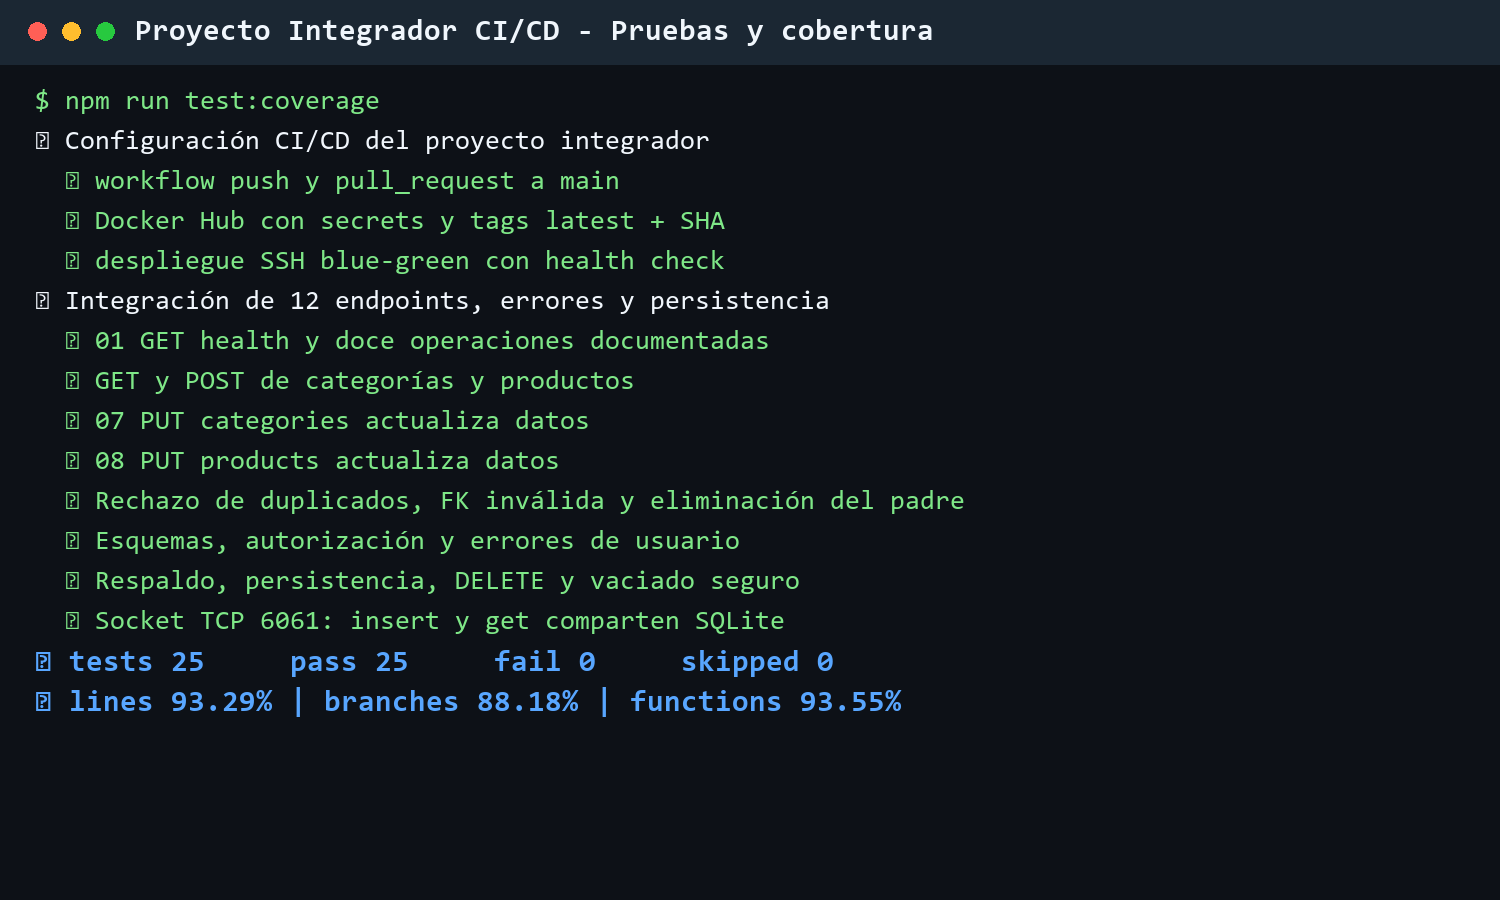
\includegraphics[width=0.96\textwidth]{evidencias/17-pruebas-unitarias-node.png}
\caption{Resumen de pruebas y cobertura ejecutado localmente el 7 de octubre de 2026.}
\label{fig:cobertura}
\end{figure}

\section{Contenedorización}
El Dockerfile utiliza \texttt{node:22.22.3-bookworm-slim}, copia únicamente los archivos necesarios, crea el volumen \texttt{/data}, cambia al usuario \texttt{node} y define un health check. El archivo \texttt{.dockerignore} adopta una lista blanca: excluye todo el contexto y permite solamente el backend, los recursos públicos y el Dockerfile. Esto evita incorporar llaves, archivos \texttt{.env}, repositorios Git, reportes o dependencias locales.

\section{Pipeline de GitHub Actions}
\begin{lstlisting}[language={},caption={Secuencia lógica del workflow principal.}]
push o pull_request a main
  -> npm run test:coverage
push aprobado a main
  -> docker login con DOCKERHUB_USERNAME y DOCKERHUB_TOKEN
  -> docker build y push de :latest y :github.sha
  -> SSH con EC2_SSH_KEY y EC2_KNOWN_HOSTS
  -> deploy-blue-green.sh
\end{lstlisting}

Los secretos requeridos son \texttt{DOCKERHUB\_USERNAME}, \texttt{DOCKERHUB\_TOKEN}, \texttt{EC2\_HOST}, \texttt{EC2\_USER}, \texttt{EC2\_SSH\_KEY}, \texttt{EC2\_KNOWN\_HOSTS} y \texttt{ADMIN\_TOKEN}. El repositorio no contiene sus valores.

\section{Despliegue continuo en EC2}
El script de despliegue selecciona el color inactivo, descarga la imagen inmutable y monta el volumen persistente de SQLite. Después de confirmar la salud de la aplicación, genera una configuración nueva de Nginx, valida su sintaxis y recarga el servicio. Finalmente registra el color activo y elimina la versión anterior. El grupo de seguridad debe permitir SSH desde la IP administrativa y HTTP en el puerto 80.

\section{Resultados}
\begin{table}[H]
\centering
\caption{Resultados verificables del proyecto.}
\begin{tabular}{p{7.2cm}p{3cm}p{4cm}}
\toprule Criterio & Resultado & Estado \\ \midrule
API REST con al menos seis endpoints & 12 operaciones & Cumplido \\
Pruebas automatizadas & 25 aprobadas, 0 fallidas & Cumplido \\
Cobertura de líneas & 93.29\% & Cumplido \\
Cobertura de ramas & 88.18\% & Cumplido \\
Cobertura de funciones & 93.55\% & Cumplido \\
Dockerfile y dockerignore & Revisión estática aprobada & Cumplido \\
Workflow push y pull request & Archivo main.yml creado & Cumplido \\
Build Docker local & Motor Docker apagado & Pendiente \\
Publicación y despliegue real & Secretos aún no configurados & Pendiente \\ \bottomrule
\end{tabular}
\end{table}

\begin{figure}[H]
\centering
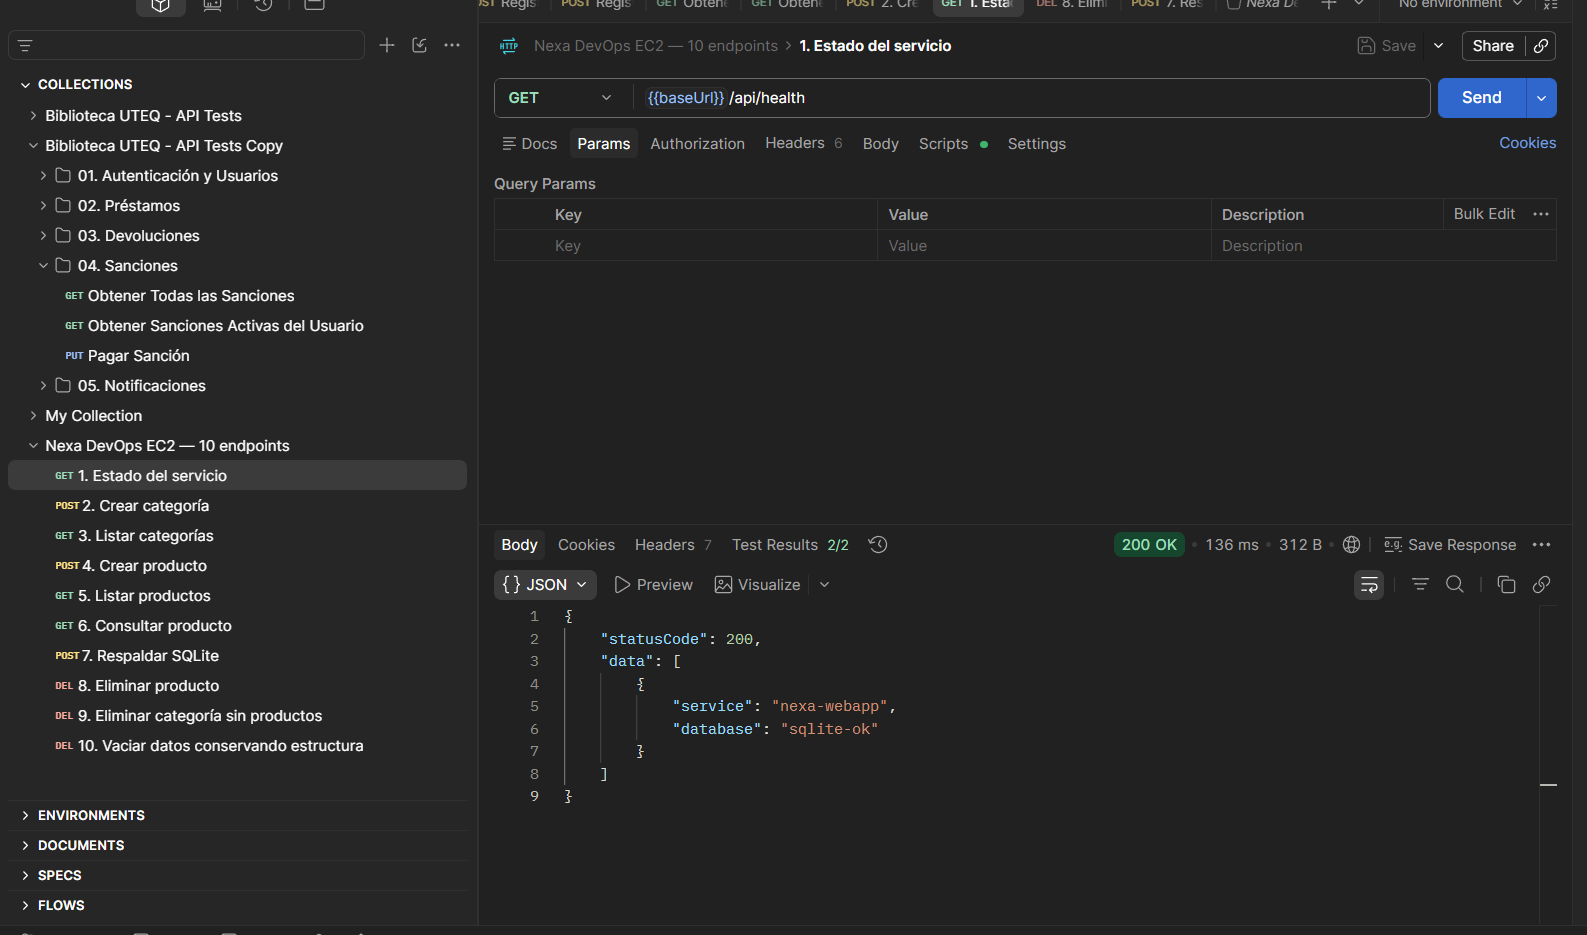
\includegraphics[width=0.96\textwidth]{evidencias/14-postman-health-aws.png}
\caption{Respuesta HTTP 200 del endpoint de salud desplegado previamente en AWS EC2.}
\label{fig:postman}
\end{figure}

La Figura~\ref{fig:postman} confirma que la API y SQLite respondieron desde EC2 en la práctica previa. Para cerrar el proyecto integrador se debe ejecutar el nuevo workflow y capturar los tres jobs aprobados, las dos etiquetas en Docker Hub y la misma URL por el puerto 80.

\section{Conclusiones}
El proyecto convirtió una API funcional en un artefacto verificable y preparado para entrega continua. La cobertura quedó ampliamente por encima del mínimo: 93.29 por ciento de líneas, 88.18 por ciento de ramas y 93.55 por ciento de funciones. Las pruebas no se limitaron a respuestas exitosas; también verificaron validación, autenticación, integridad de SQLite, respaldo, persistencia y estructura de CI/CD. Esta combinación reduce la probabilidad de publicar una versión que falle por errores conocidos.

La estrategia blue-green separa la construcción de la activación. La imagen nueva debe responder correctamente antes de recibir tráfico y Nginx puede cambiar de destino mediante una recarga, lo que evita detener primero la versión saludable. La seguridad se mantiene al usar GitHub Secrets, una etiqueta inmutable por commit, validación de \texttt{known\_hosts}, ejecución sin privilegios y un archivo de entorno protegido en EC2. Quedan como pasos operativos encender Docker Desktop y registrar los secretos; una vez realizados, un \texttt{git push} a \texttt{main} demostrará el ciclo completo solicitado.

\section{Fuentes de información}
\begin{enumerate}
\item GitHub. \textit{Understanding GitHub Actions}. \url{https://docs.github.com/actions}
\item Docker. \textit{Build and push Docker images}. \url{https://docs.docker.com/build/ci/github-actions/}
\item Docker. \textit{Personal access tokens}. \url{https://docs.docker.com/security/access-tokens/}
\item Amazon Web Services. \textit{Get started with Amazon EC2}. \url{https://docs.aws.amazon.com/AWSEC2/latest/UserGuide/EC2_GetStarted.html}
\item Node.js. \textit{Test runner and code coverage}. \url{https://nodejs.org/api/test.html}
\end{enumerate}
\end{document}
